
%% LaTeX2e class for technical reports
%% techreport.tex
%% 
%% Karlsruhe Institute of Technology
%% Institute for Program Structures and Data Organization
%% Chair for Software Design and Quality (SDQ)
%%
%% Dr.-Ing. Erik Burger
%% burger@kit.edu
%%
%% See https://sdq.kastel.kit.edu/wiki/Dokumentvorlagen
%%
%% Version 1.0, 2023-11-20

%% Available page modes: oneside, twoside
%% Available languages: english, ngerman
%% Available modes: draft, final (see README)
\documentclass[oneside, english]{reports/assets/sdqtechreport}

%% ---------------------------------
%% | Information about the thesis  |
%% ---------------------------------

%% Name of the author
\author{Konstantin Bernhard \and Klim Petraschkevich \and Kristiyan Skordev \and Felix Uhlenbrock \and Justus Zorn}

%% Title (and possibly subtitle) of the thesis
\title{Intrusion Detection using Machine Learning}
\subtitle{Specification}


%% You can put a logo in the ``logos'' directory and include it here
%% instead of the SDQ logo
% \grouplogo{myfile}
%% Alternatively, you can disable the group logo
\nogrouplogo

\date{\today}

\usepackage{graphicx}
\graphicspath{ {./reports/assets} }

%% ====================================
%% ====================================
%% ||                                ||
%% || Beginning of the main document ||
%% ||                                ||
%% ====================================
%% ====================================
\begin{document}

%% Set PDF metadata
\hypersetup{
	pdftitle = {Specification},
	pdfsubject = {Intrusion Detection using Machine Learning},
	pdfauthor = {Konstantin Bernhard, Klim Petraschkevich, Kristiyan Skordev, Felix Uhlenbrock, Justus Zorn}
}

%% Set the title
\maketitle

%% ------------------------
%% |   Table of Contents  |
%% ------------------------
\tableofcontents

%% -----------------
%% |   Main part   |
%% -----------------
\cleardoublepage

%% -------------------
%% | Example content |
%% -------------------

\chapter{Alerts}
\label{chap:Alerts}
Alerts are used to notify the administrator of suspicious activity, even while
the administrator is not actively checking the IDS or even working at all.

\section{Alert Content}
\label{sec:AlertContent}
Since the administrator might not be working when they receive an alert, the
alert MUST include all information necessary for the administrator to take
action, including:
\begin{itemize}
	\item The exact time and date of the attack, so that the administrator knows
	whether it is still in progress or already over.
	\item The type and severity of the attack, since certain attacks (e.g. DoS)
	only cause downtime, while others (e.g. SQL injection) can cause data leakage
	and are therefore much more problematic.
	\item How certain the IDS is that this is an actual attack, instead of normal
	behavior. This is especially important since an administrator may take
	actions in response to threats that are themselves a threat to the network,
	e.g. shutting down servers immediately (which might cause data loss and
	downtime). If the IDS provides a certainty score (between 0 and 1), the
	administrator knows whether they should inspect the attack more closely first
	or take action immediately.
	\item A hyperlink to a webpage (in the user interface, if developed)
	that contains further information about the exact notification the
	administrator received.
\end{itemize}

\section{Alert Delivery}
\label{sec:AlertDelivery}
It is likely that most attacks happen while the administrator is not paying
close attention to the system, so it is essential that the alerts are
delivered within a couple of seconds and that they are loud enough to alarm
the administrator, potentially even during the night. Otherwise, the attack
might be over before the administrator even notices that anything happens.

The obvious choice for alert delivery is a messenger, which is typically
installed on mobile devices. Since messengers are used for asynchronous
communication between people, they often include functionality to notify
the user, even while not looking at the device. Typical ways of achieving
this are a notification sound or vibration.

Many messengers, especially those built for communication in bigger teams,
include functionality to send messages automatically, i.e. from other services.
This is achieved using webhooks, which means that the messenger service is
listening on the network, and our IDS can send a request via the HTTP
protocol, which will then send a message to the intended user. Common examples
of messengers implementing such functionality are Mattermost, Slack, and Teams.

To make our IDS more flexible and not fix it to a certain messenger service, it
MUST have the ability to send webhook requests to arbitrary servers, which can
be configured by the administrator. These webhook requests MUST be in the JSON
data format, and sent via the HTTP POST protocol to a user-provided URL. The
structure of the requests is as follows:

\begin{verbatim}
{
	"timestamp": <UNIX time stamp>,
	"attack": <name of attack>,
	"severity": <one of low, medium, high>,
	"certainty": <score between 0 and 1, 0: uncertain, 1: certain>,
	"link": <link to a webpage with further details, if implemented>
}
\end{verbatim}

The exact names of the attacks as well as the assigned severities and
certainties depend on the database used for the IDS. The administrator can
write a service themselves which provides a webhook and configure the IDS to
send all alerts to this webhook. This service will then be responsible for
parsing the above datastructure, and sending webhooks to the actual messenger
services. While this is more effort for the administrator, it makes the IDS
completely independent of the messenger service used for delivering the alerts
to the user. If possible, the project SHOULD contain at least one example for
such a service which delivers alerts to an actual messenger service.

\begin{center}
	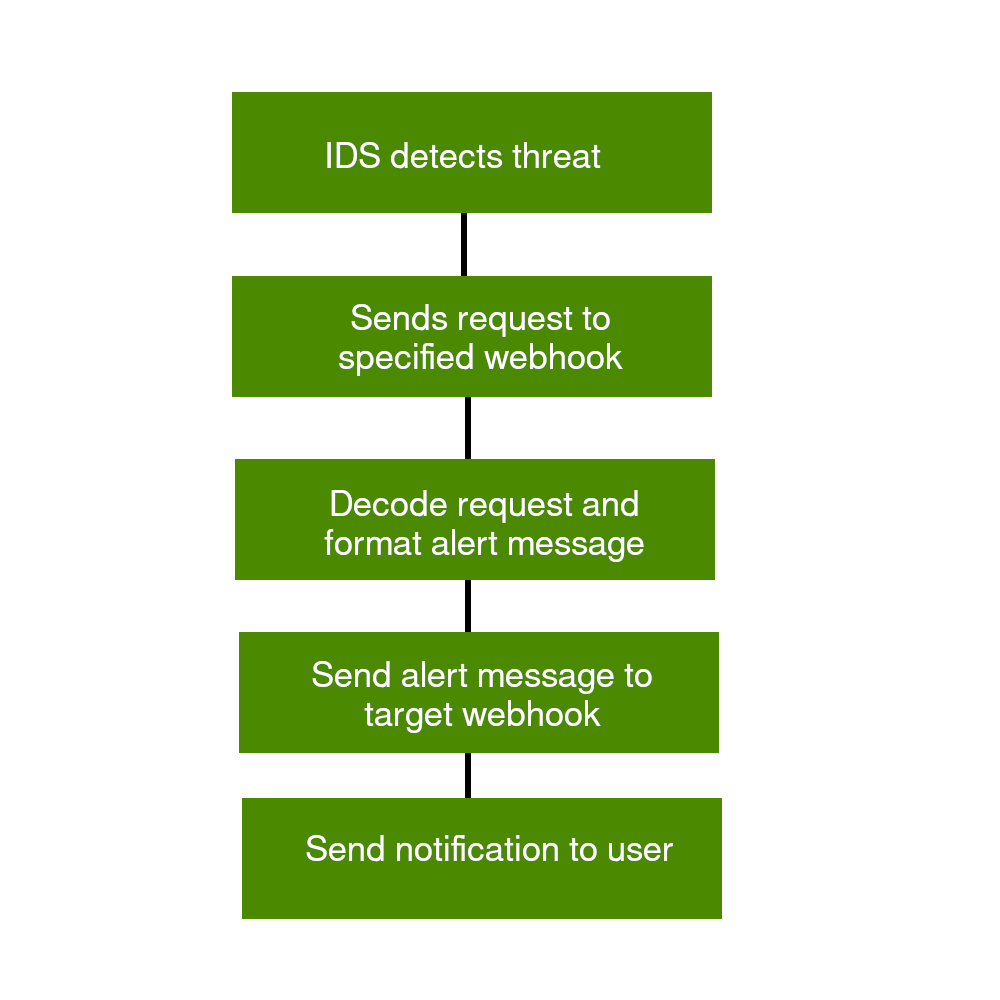
\includegraphics{alert-workflow}
\end{center}

\chapter{User Interface}
\label{chap:UserInterface}

While not essential to our project, the IDS SHOULD contain a user interface
that provides the administrator with deeper insights into their network. The
user interface SHOULD be provided as a simple website, served directly from
the main deployment, i.e. there MUST be no separate website server.

The UI SHOULD consists of three different parts:
\begin{itemize}
	\item An overview of the system
	\item Detail pages for the individual alerts
	\item Configuration options for the IDS
\end{itemize}

\section{Overview}
\label{sec:UserInterfaceOverview}

The overview MUST contain some statistics to assess health, including but not
limited to:
\begin{itemize}
	\item The total number of packets processed, so the administrator can easily
	assess whether the system is overloaded.
	\item The average duration packet processing takes, so the administrator can
	detect when the IDS itself is overloaded.
	\item The amount of alerts sent, and how many of these were marked as correct
	by the administrator. This can help the administrator to adjust settings
	related to the false-positive rate of the IDS.
\end{itemize}

Also, the overview MUST contain a list of currently active alerts, which is all
alerts that were triggered but not yet reviewed by the administrator. This list
MUST contain exactly the information that is also present in the alert HTTP
requests, as specified in section \ref{sec:AlertDelivery}. Clicking on a single
alert leads to the alert display page specified in section
\ref{sec:UserInterfaceAlertDetails}.

\section{Alert Details}
\label{sec:UserInterfaceAlertDetails}

The alert details MUST contain the information already provided in the alert
itself, i.e.
\begin{itemize}
	\item Timestamp
	\item Attack type
	\item Attack severity
	\item Certainty
\end{itemize}

It MAY also contain further descriptions:
\begin{itemize}
	\item An overview of the attack, in case the administrator is not familiar
	with it. This description MAY be sourced from a database, or generated by the
	system automatically.
	\item An estimate of the effect the attack would have, which explains the
	severity. This may e.g. include whether the IDS estimates the attack would
	succeed, or which services could be affected.
	\item A proposed plan of action. This MAY also be sourced from a database, or
	generated by the IDS. In any case, the IDS should never perform such actions
	automatically, and the administrator should only view this plan of action as a
	hint, and not rely on it.
\end{itemize}

The alert details page MUST include buttons for reviewing the attack:
\begin{itemize}
	\item Dismiss: When the administrator clicks this button, the alert is removed
	from the active alert list on the overview page. This information SHOULD be
	used to train the IDS or adjust the settings, so that the number of false
	positives may be reduced.
	\item Resolved: When the administrator clicks this button, the alert is
	also removed from the active alert list. This information MAY also be used to
	further train the IDS.
\end{itemize}

The page MAY include a text field for notes the administrator can use to
associate information with this specific type of attack, or the alert itself.

\section{Settings}
\label{sec:UserInterfaceSettings}

The settings page allows the administrator to configure how the IDS works:

\begin{itemize}
	\item It MUST provide a way to configure the webhook URL,
	which determines where alerts are sent. This is specified in section
	\ref{sec:AlertDelivery}.
	\item It SHOULD provide a minimum certainty level, which allows the
	administrator to adjust how certain the IDS has to be before sending an alert.
	This is important to adjust the false-positive rate to an acceptable level.
	\item It SHOULD provide options specific to the exact model used by the IDS.
	\item It MAY provide a list of previously reviewed alerts, and the option to
	change the review of these (in case the review was wrong).
	\item It MAY provide a way to add signatures or similar to influence the
	decision-making process of the IDS directly.
\end{itemize}

\section{Preliminary Designs}
\label{sec:UserInterfaceDesigns}

Overview page:

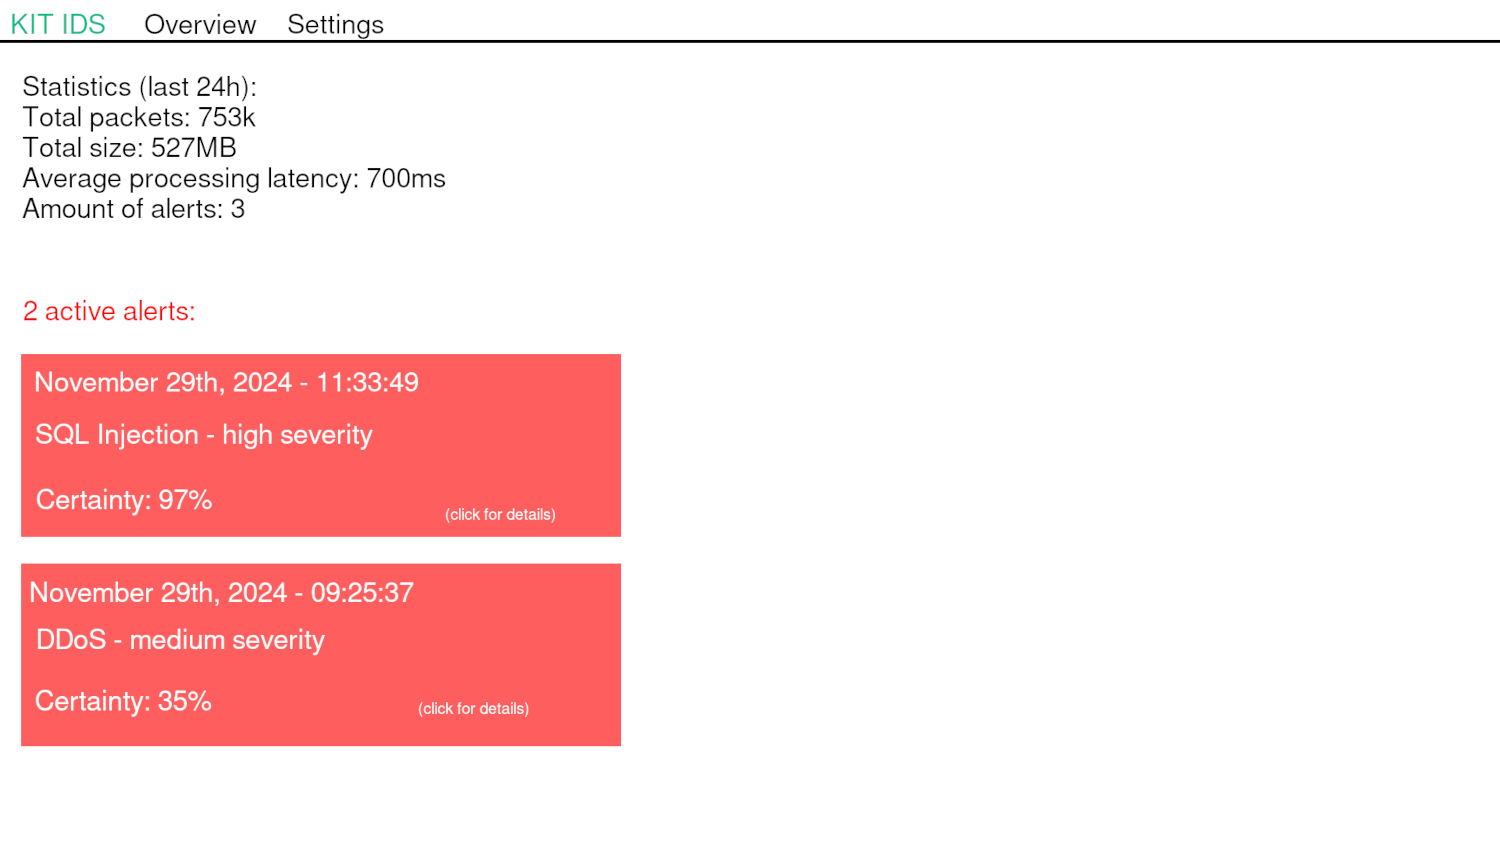
\includegraphics{ui-overview}

Alert details page:

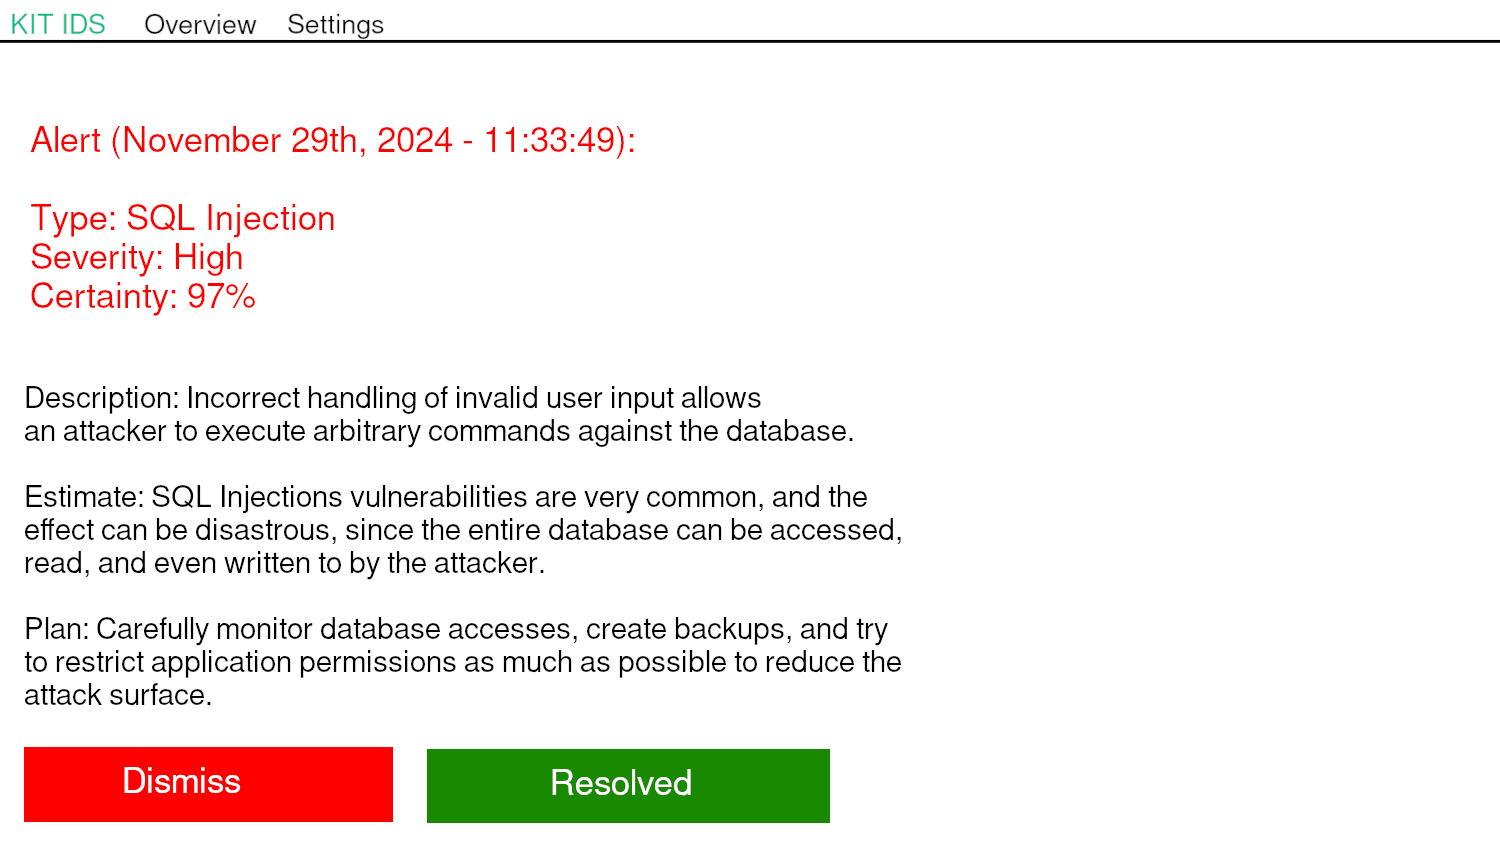
\includegraphics{ui-details}

Settings page:

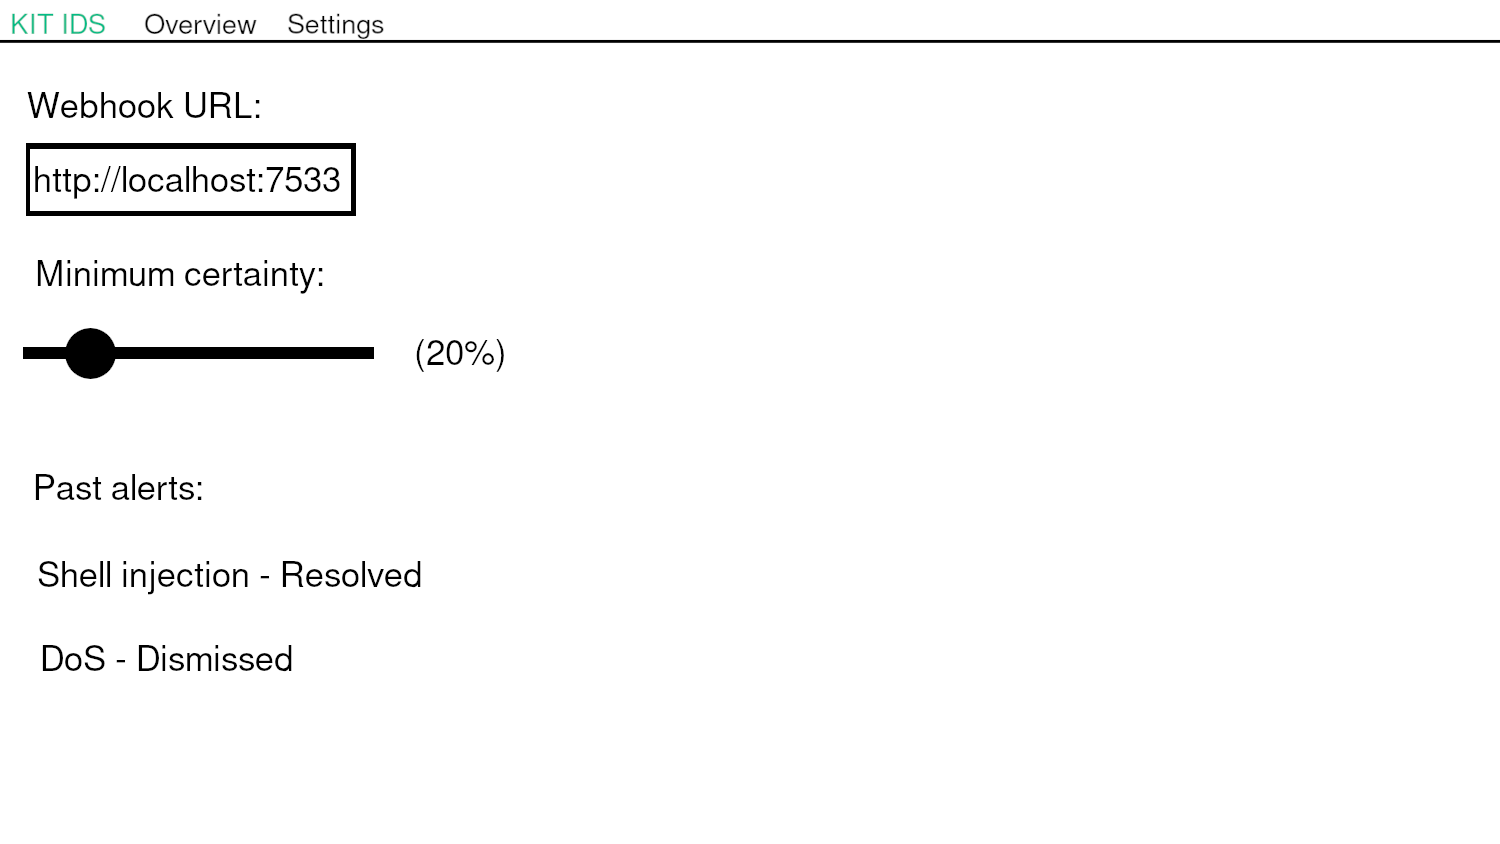
\includegraphics{ui-settings}

\end{document}

